\section{Methods}
\label{sec:methods}
GeoEvidence-RAG answers a drawing question by constructing a set of citable records. The question determines both the observations needed for a local judgment and the population needed for a collection claim. Figure~\ref{fig:method-map} places these decisions within the study.

\begin{figure}[!ht]
\centering
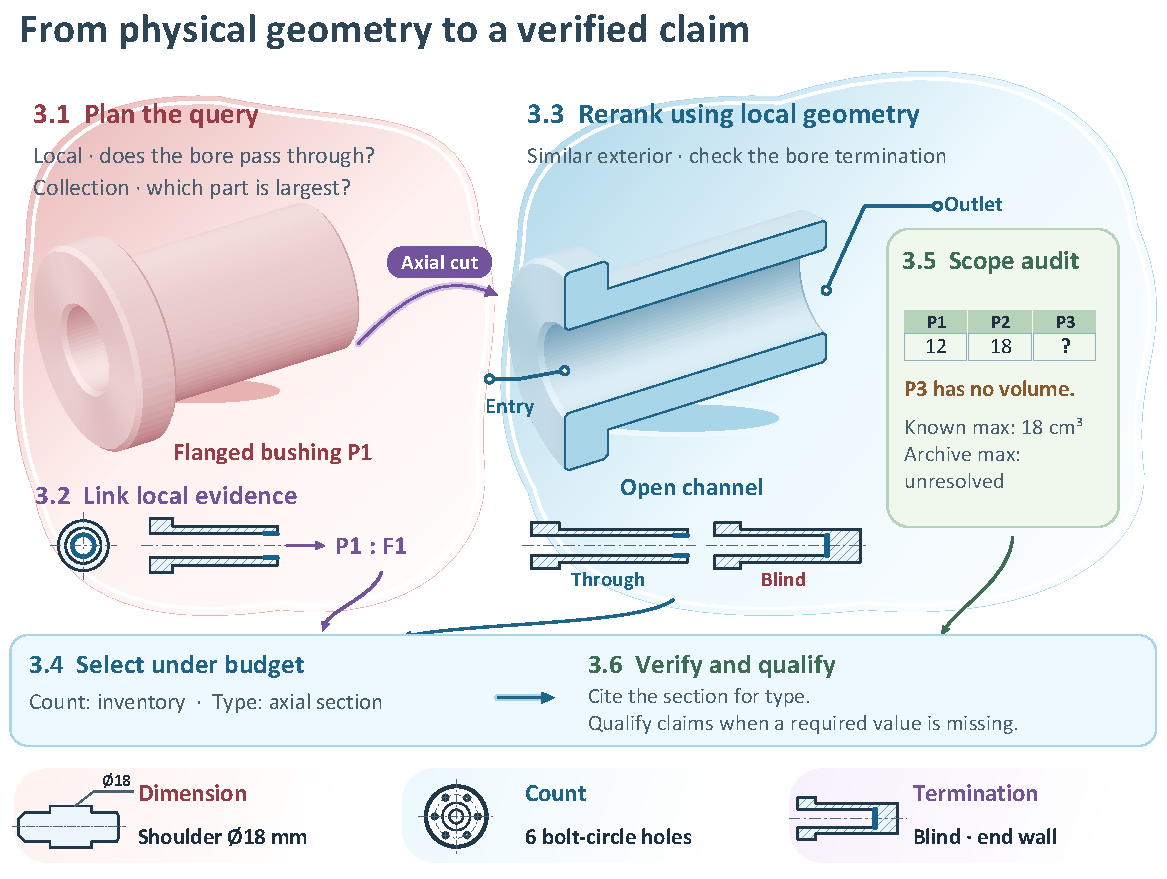
\includegraphics[width=\linewidth]{figures/study-plate.pdf}
\caption{The six method stages around a flanged bushing. The synthetic cutaway identifies the entry and outlet that support a local termination claim. The registry illustrates a different requirement: removing P3's volume in Step~3 of Figure~\ref{fig:geoevidence-comparison}B leaves the collection maximum unresolved. Both kinds of record enter budgeted selection and claim verification. The bottom examples illustrate dimension readout, feature counting, and termination judgment.}
\label{fig:method-map}
\end{figure}

\subsection{Problem definition}
\label{sec:problem}
Let $q$ be a question over an archive of drawing observations and, where available, native CAD attributes. We maintain an evidence index $\mathcal E$ and a registry $\mathcal P$ of part identifiers. The registry records the parts eligible under the declared scope, including parts whose attributes are missing. For a given part $p$, the index supplies the records
\begin{equation}
  \mathcal E_p=\{e\in\mathcal E:p(e)=p\}.
\end{equation}
A query plan specifies a nonempty set of conditions $C$, a scope, and an optional aggregate operator. A request for the largest part by volume, for example, specifies a property, a population, and a maximum operator:
\begin{equation}
  \operatorname{plan}(q)=(C,\operatorname{scope}(q),\operatorname{op}(q)).
\end{equation}
The reader receives a set $S$ drawn from a candidate pool $U$. The context budget $B$ bounds the sum of the positive record costs $b(e)$:
\begin{equation}
  S\subseteq U,\qquad b(S)=\sum_{e\in S}b(e)\le B .
  \label{eq:method-budget}
\end{equation}
Every engineering judgment $j$ carries its condition identifiers $C_j$ and its cited evidence identifiers $I_j$. The result is an answer with a claim-level audit trail:
\begin{equation}
  \operatorname{output}(q)=
  \bigl(\operatorname{answer},\,\{(j,C_j,I_j)\}_{j\in\operatorname{claims}}\bigr).
\end{equation}
Table~\ref{tab:method-notation} lists the notation shared across stages.

Consider two requests about the bushing in Figure~\ref{fig:method-map}. To determine whether its central bore passes through the part, the relevant observations concern one identified feature. A section through the bore axis can settle the question if it shows the channel meeting both exterior faces. To identify the bushing with the largest volume in an archive, every eligible part contributes a potential counterexample. Adding an omitted part can change the winner even if every previously read dimension was correct. This difference determines how $U$ is assembled before the budget in Eq.~\eqref{eq:method-budget} is applied.

The distinction between $U$ and $S$ also matters for a question with several clauses. Suppose the reader is asked for both a bore diameter and its termination. A diameter annotation supports a size claim, while a section establishes where the channel ends. Giving each judgment its own $C_j$ and $I_j$ makes it possible to identify a missing sectional observation even when the diameter has been read correctly. The budget controls what the reader sees. The population named in the question remains the same.

\begin{table}[!htbp]
\centering
\caption{Notation used across the method.}
\label{tab:method-notation}
\small\vspace{4pt}
\renewcommand{\arraystretch}{1.08}
\begin{tabular}{@{}l@{\hspace{1em}}p{.67\linewidth}@{}}
\hline
Symbol & Meaning \\ \hline
$q,\ C,\ c$ & Question, its verification conditions, and one condition.\\
$\mathcal P,\ p,\ f$ & Declared part registry, part identifier, and feature identifier within a part.\\
$\mathcal E,\ e$ & Evidence index and one citable record.\\
$F,\ R,\ A,\ L$ & CAD faces, view regions, attributed properties, and source locators of a record.\\
$K,\ U,\ S$ & Candidate depth, available evidence pool, and selected evidence.\\
$B,\ b(e)$ & Context budget and positive cost of record $e$.\\
$h(e,c),\ H_c(S)$ & Support for condition $c$ from one record and best support in $S$.\\
$w_c,\ \lambda$ & Condition weight and redundancy penalty.\\
$a,\ D_a$ & Requested attribute and parts with a usable value for it.\\
$j,\ C_j,\ I_j$ & Answer claim, attached conditions, and cited identifiers.\\
\hline
\end{tabular}
\end{table}

\FloatBarrier
\subsection{Construction of local geometric evidence units}
\label{sec:method-units}
Each property stays attached to the feature it describes. Each feature record carries a stable key $(p,f)$, face identifiers $F$, regions $R$, a property map $A$, and source locators $L$:
\begin{equation}
  e=(p,f,F,R,A,L),\qquad \operatorname{id}(e)=(p,f).
\end{equation}
The record also stores its type and cost. An empty $F$ is admissible for a drawing-only record. Each region identifies a view, an image and a normalized box. For a crop with page bounds $(x_0,y_0,x_1,y_1)$, a crop-relative point $(u,v)$ maps back to
\begin{equation}
  T(u,v)=\bigl(x_0+(x_1-x_0)u,\;y_0+(y_1-y_0)v\bigr).
\end{equation}
Applying $T$ to the two box corners recovers a location on the original page. Boxes from different projections may occupy unrelated coordinates. Their grouping instead uses the identity assigned to each input record $r$:
\begin{equation}
  G_{pf}=\{r:(p(r),f(r))=(p,f)\}.
\end{equation}
The coordinate transform can be audited independently of feature interpretation. Consider a crop spanning $(0.20,0.10)$ to $(0.60,0.50)$ on the page. A detection from $(0.25,0.25)$ to $(0.75,0.75)$ inside that crop maps to $(0.30,0.20)$ and $(0.50,0.40)$ on the sheet. Applying $T$ once allows the reader to revisit the source location even if the crop was resized for retrieval. Identifying the same physical bore in a different projection requires the separate correspondence key $(p,f)$.

\begin{figure}[!ht]
\centering
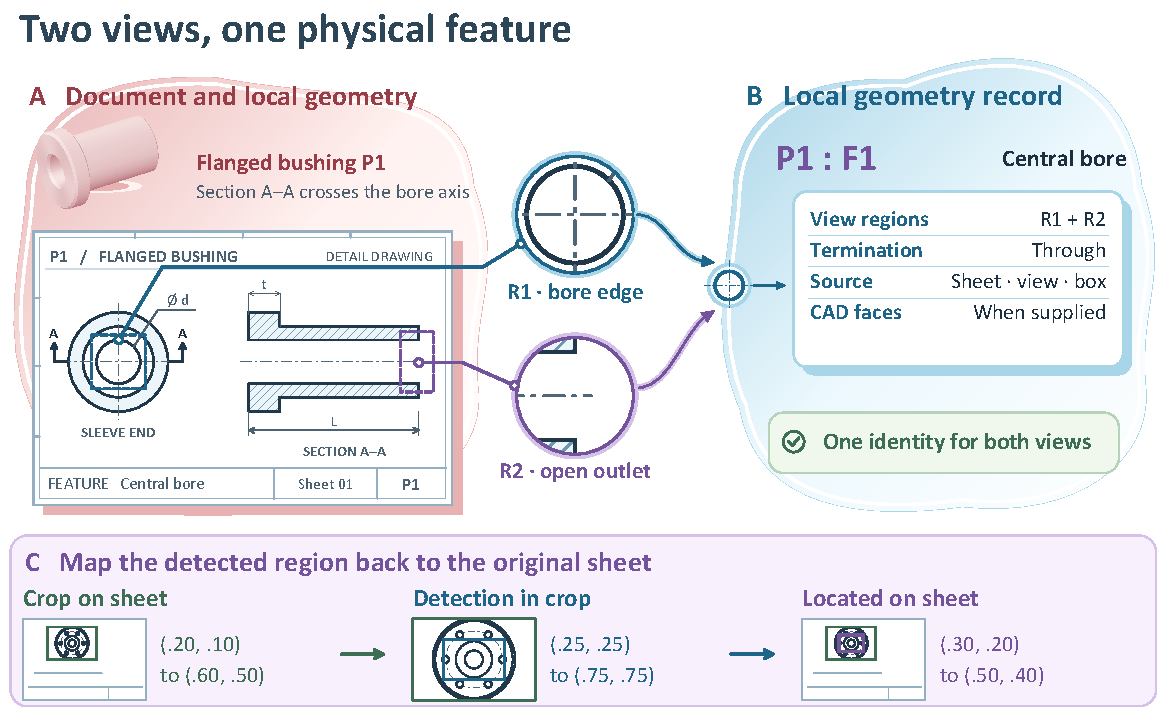
\includegraphics[width=\linewidth]{figures/feature-record-plate.pdf}
\caption{Construction of a local geometric evidence unit. (A) Detail windows enlarge the marked bore edge and outlet from the same source drawing. (B) The key P1:F1 retains both view locators and the observed termination. (C) A separate coordinate example follows a detection from a cropped view back to its original sheet. Each pair of coordinates specifies a corner of the normalized box.}
\label{fig:method-unit}
\end{figure}

Within a group, the merge pools the face, region, and source sets, retaining distinct view locators:
\begin{equation}
 (F,R,L)_{pf}=
 \left(\bigcup_{r\in G_{pf}}F_r,\ \bigcup_{r\in G_{pf}}R_r,\
       \bigcup_{r\in G_{pf}}L_r\right).
\end{equation}
Common keys in $A$ must agree. Categorical values require equality. Numeric values $u,v$ in the same units agree when
\begin{equation}
 |u-v|\le \max\{\epsilon,\epsilon\max(|u|,|v|)\}.
\end{equation}
The default merge tolerance is $\epsilon=10^{-6}$ in the stored units. Conflicting properties or identity metadata cause the merge to fail. Figure~\ref{fig:method-unit} shows how two projections retain distinct roles after consolidation. Assigning the shared key requires a source correspondence. Similar contours alone leave the identity unresolved.

The bushing illustrates the ambiguity. Several circles share a center in the sleeve-end view, yet their boundaries belong to the bore, the sleeve exterior, or the flange. Attaching the bore diameter to the flange edge would preserve a plausible numeric value under the wrong owner. Keeping the individual locators after consolidation lets an inspector follow a dimension back to its referenced edge and a termination judgment back to its sectional contour. The merge tolerance $\epsilon$ governs agreement between stored values. A manufacturing tolerance attached to a dimension is a separate engineering property with its own source.

\subsection{Global candidate search and modeling of local geometric differences}
\label{sec:method-rank}
For a visual query profile, let $z_q$ and $z_p$ denote the reference and candidate part embeddings from a frozen CLIP encoder~\cite{radford2021clip}. The first stage retrieves the $K$ highest cosine scores:
\begin{equation}
 g_p=\frac{z_q^\top z_p}{\|z_q\|\,\|z_p\|},\qquad
 P_K=\operatorname{TopK}_{p\in\mathcal P}\,g_p .
\end{equation}
Zero-norm vectors receive score zero. Text-only queries can supply candidate identifiers directly. Pairwise geometric reranking requires a reference profile and candidate profiles.

For each query feature $f$ with embedded regions, compare its crops with candidate crops of the same feature type. With $z_r$ the embedding of region $r$ and $R_p$ the candidate's embedded regions, the best available alignment is
\begin{equation}
 d_f(p)=\max_{\substack{r\in R_f,\ t\in R_p\\
                   \operatorname{type}(t)=\operatorname{type}(f)}}
                   \cos(z_r,z_t).
\end{equation}
Let $M$ contain features with a matched score above $-1$, and let $n$ count query features with embedded regions. Three statistics summarize the strength and extent of alignment:
\begin{equation}
 d_{\max}=\max_{f\in M}d_f,\qquad
 \bar d=\frac{1}{|M|}\sum_{f\in M}d_f,\qquad
 \rho_f=\frac{|M|}{n}.
\end{equation}
For critical attribute $a$, let $A_p[a]$ denote the set of its observed values across the part. On the keys $J$ observed for both profiles, the agreement and disagreement fractions are
\begin{equation}
 m_+=\frac{\sum_{a\in J}\mathbf1\{A_q[a]=A_p[a]\}}{|J|},\qquad
 m_-=\frac{\sum_{a\in J}\mathbf1\{A_q[a]\ne A_p[a]\}}{|J|}.
\end{equation}
Empty pools and zero denominators in these summaries return zero. If $v_q,v_p$ count distinct views, $\rho_v=\min(1,v_p/\max(1,v_q))$ measures view availability. The learned score uses seven inputs:
\begin{equation}
 x_p=(g_p,d_{\max},\bar d,m_+,m_-,\rho_f,\rho_v),\qquad
 s_p=\sigma\!\left(\operatorname{MLP}_{\theta}(x_p)\right).
\end{equation}
The MLP has two ReLU hidden layers of widths 16 and 8. A fixed weighted scorer over $x_p$ is available when a trained checkpoint is absent. Candidate parts are ordered by the chosen score before their evidence is collected.

Two bushings can have nearly identical $g_p$ because their outer envelopes and front openings match. Their strongest crop scores $d_{\max}$ may also be close when the best pair depicts only the opening. Suppose hole count and bore type are the only comparable attributes. For a through-bore reference, a blind-bore candidate with the correct count gives $(m_+,m_-)=(0.5,0.5)$, while a candidate matching both properties gives $(1,0)$. The scorer can use this distinction even when the global descriptor changes little. If bore type is missing, it drops out of $J$ and agreement on count alone can again give $m_+=1$. A high score in that case warrants inspection of a sectional record before making a claim about termination.

Training pairs are mined among visual neighbors. A weak label compares their full critical-attribute signatures $\operatorname{sig}$ when at least one critical value is observed across the pair:
\begin{equation}
 y_{qp}=\mathbf1\{\operatorname{sig}(q)=\operatorname{sig}(p)\}.
\end{equation}
A change from a blind bore to a through bore can yield a negative pair at high $g_p$. Unequal annotation completeness can also yield $y_{qp}=0$. For an editable CAD variant, a controlled pair requires regenerating the affected views and descriptors after the edit. Binary cross-entropy trains the reranker:
\begin{equation}
 \mathcal L(\theta)=-\operatorname{mean}_{(q,p)}
 \big[y_{qp}\log s_p+(1-y_{qp})\log(1-s_p)\big].
\end{equation}
Here $\sigma$ is the logistic function. Only $\theta$ is optimized. An original part, its variants and their projections inherit one family identifier. Writing $\mathcal F$ for sets of families, the split enforces
\begin{equation}
 \mathcal F_{\rm train}\cap\mathcal F_{\rm test}=\varnothing .
\end{equation}
A pair enters a partition only when both endpoints belong to it. Pairs crossing the boundary are discarded.

The matching rule explains why feature identity is still needed downstream. Two query features can attain their largest crop similarities against the same candidate region, since the maxima in $d_f(p)$ are computed independently. Thus $\rho_f$ measures the availability of plausible matches and cannot establish a one-to-one correspondence for counting. Similarly, renderings of one edited part can produce many nearly identical test pairs. Holding out the entire family makes ranking evaluation sensitive to transfer across parts. First-stage recall sets a further limit on this evaluation because a reranker can reorder only the parts present in $P_K$.


\subsection{Question decomposition and complementary evidence selection under a budget}
\label{sec:method-selection}
A rule-based parser matches property aliases in $q$ and identifies an operator such as maximum, minimum, ordering, or distinct count. A named property normally gives one condition. If none is recognized, the normalized question becomes a descriptive condition. Each condition carries its requested keys, priority, and an exhaustive-scope flag:
\begin{equation}
 c=(\operatorname{keys}(c),w_c,\operatorname{scope}(c),
             \operatorname{exhaustive}(c)).
\end{equation}
Figure~\ref{fig:method-budget} illustrates the marginal gain for two requested properties.

\begin{figure}[!ht]
\centering
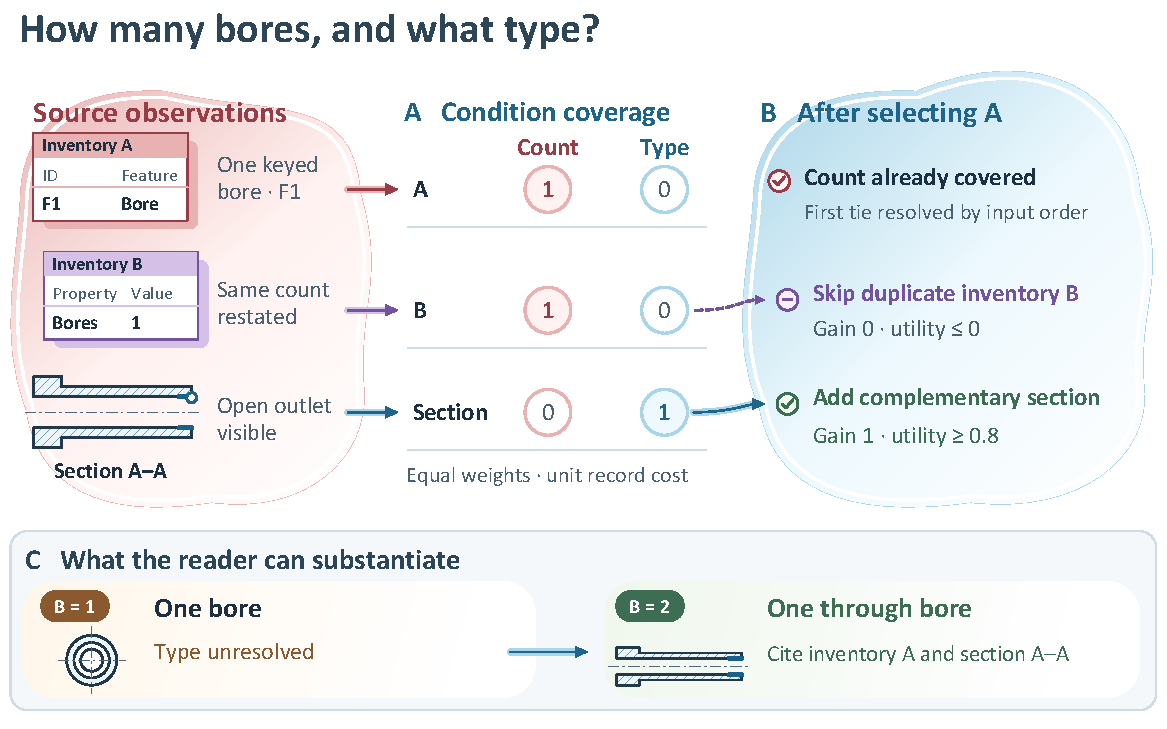
\includegraphics[width=\linewidth]{figures/selection-plate.pdf}
\caption{Complementary evidence selection for an illustrative part with one bore. The source excerpts show two inventories and an axial section. (A) The inventories cover the same count condition. (B) Input order breaks the initial tie. With unit costs, equal weights, and $\lambda=0.2$, adding the section after inventory A has utility at least $0.8$. (C) A one-record answer leaves termination open. At two records, the reader can cite both count and type.}
\label{fig:method-budget}
\end{figure}

For a local condition, $h(e,c)$ measures how much relevant information a record exposes. Write $J_c=\operatorname{keys}(c)$ and let $T_c,T_e$ be the token sets of the description and of the record summary plus feature type. The default support score is
\begin{equation}
 h(e,c)=
 \begin{cases}
 |J_c\cap\operatorname{keys}(A_e)|/|J_c|,&J_c\ne\varnothing,\\
 |T_c\cap T_e|/\max(1,|T_c|),&J_c=\varnothing .
 \end{cases}
\end{equation}
Property presence indicates that an observation can be inspected. Its value still determines the engineering answer. For an exhaustive condition, only a structured aggregate for the requested attribute receives credit:
\begin{equation}
 h(e,c)=
 \begin{cases}
 1,&\text{matching aggregate with complete scope},\\
 0.4,&\text{matching aggregate with incomplete scope},\\
 0,&\text{otherwise}.
 \end{cases}
 \label{eq:aggregate-support}
\end{equation}
The partial score lets a bounded context carry an explicit warning. Each condition retains the strongest selected support, initialized at zero:
\begin{equation}
 H_c(S)=\max\bigl(\{0\}\cup\{h(e,c):e\in S\}\bigr).
\end{equation}
Writing $[u]_+=\max(0,u)$, the additional weighted coverage offered by a candidate is
\begin{equation}
 \Delta(e\mid S)=\sum_{c\in C}w_c\,[h(e,c)-H_c(S)]_+ .
\end{equation}
A request for both hole count and bore type illustrates the choice of decomposition. With separate conditions $c_1$ and $c_2$, an inventory can fully support $c_1$ and a section can fully support $c_2$. If both keys were bundled into one condition, each record would score $1/2$ and their maximum would remain $1/2$ after both were selected. The maximum in $H_c(S)$ therefore favors conditions that can each be verified from one record. Properties that must hold for the same bore still require an identity check. Two units from different parts may cover both property names without answering the joint question about P1.

Redundancy uses Jaccard overlap $J(X,Y)=|X\cap Y|/|X\cup Y|$, with zero for an empty union. For distinct records $e,t$, let $i_p$ indicate a shared part and $i_t$ a shared feature type. With $T'_e$ denoting summary tokens, define
\begin{equation}
 r(e,t)=\max\{i_p J(F_e,F_t),\,J(T'_e,T'_t),\,0.5\,i_p i_t\}.
\end{equation}
Identical identifiers give $r(e,t)=1$. With a default $\lambda=0.2$, the priority of a feasible record is its net marginal gain per unit cost:
\begin{equation}
 u(e\mid S)=
 \frac{\Delta(e\mid S)-\lambda\max_{t\in S}r(e,t)}{b(e)} .
\end{equation}
The redundancy term is zero for $S=\varnothing$. Starting from that set, the selector takes the highest positive priority that fits:
\begin{equation}
 e^* \in \underset{\substack{e\in U\setminus S\\b(S)+b(e)\le B}}{\arg\max}\ u(e\mid S),
 \qquad S\leftarrow S\cup\{e^*\}\quad\text{if }u(e^*\mid S)>0 .
\end{equation}
Selection stops when all $H_c(S)=1$, the feasible set is empty, or its best gain is nonpositive. The reported coverage is the unweighted mean of $H_c(S)$.

In Figure~\ref{fig:method-budget}, taking inventory A changes the coverage vector from $(0,0)$ to $(1,0)$. Inventory B then has $\Delta=0$ even if its wording closely matches the question. For the sectional record, $\Delta=1$ and $b(e)=1$, so with $\lambda=0.2$ its utility is at least $0.8$ for any admissible redundancy score. At $B=2$ the section fits and the final vector is $(1,1)$. Reducing the budget to $B=1$ leaves bore type unresolved. Reporting the uncovered condition identifies the observation lost to the budget. Equal priorities can make the choice order-dependent, and greedy selection need not yield the globally best subset.



\subsection{Global candidate-set completeness and missing-attribute checks}
\label{sec:method-scope}
A global maximum is a statement about $\mathcal P$. Even perfect ranking within $P_K$ gives no account of an omitted part. For a recognized operator with a single attribute $a$, the structured path scans the registry independently of $K$. Assume consistent units and attribute semantics at ingestion. Define the observed and missing populations by
\begin{equation}
 D_a=\{p\in\mathcal P:\text{a usable value }a(p)\text{ is recorded}\},
 \qquad M_a=\mathcal P\setminus D_a .
\end{equation}
For numerical comparisons, a usable value must be numeric and applicable to the specified part. Repeated consistent values produce one row per part. Incompatible values raise a conflict. Let $d=1$ signify that the registry was declared complete for this scope. The completeness flag is
\begin{equation}
 \operatorname{complete}(a)=
 \mathbf1\{d=1,\ |\mathcal P|>0,\ M_a=\varnothing\}.
 \label{eq:method-complete}
\end{equation}
The registry flag and the missing set test independent assumptions. An index built solely from records containing a volume would make $M_a$ empty by construction. A separately declared list of eligible parts allows a drawing with no volume entry to remain visible during the scan. Conversely, all known parts may have values while the archive itself is only a sample. In that case $d=0$ prevents promotion of a sample maximum to a collection-wide claim.

Usability also depends on the meaning of $a$. Part volume and bounding-box volume may both be expressed in cubic millimetres, but changing an internal bore can alter one while leaving the other unchanged. The index therefore distinguishes their property keys. Comparable units are an ingestion requirement for numeric comparisons. A value whose units have not been resolved cannot justify an exact physical comparison merely because it can be parsed as a number.

The scan preserves the part identifier, value, and source evidence identifier in each row. For a maximum with $D_a\ne\varnothing$, its value and tied winners are
\begin{equation}
 v^*=\max_{p\in D_a}a(p),\qquad
 W=\{p\in D_a:a(p)\simeq v^*\},
\end{equation}
where $\simeq$ uses numerical comparison tolerance. Minima reverse the comparison. Ordering retains the per-part rows, and a distinct count groups equal attribute values. The result is packaged as one citable record $e_a$ with provenance and a completeness flag. The reader's candidate pool becomes
\begin{equation}
 U=\left(\bigcup_{p\in P_{\rm kept}}\mathcal E_p\right)\cup\{e_a\},
\end{equation}
where $P_{\rm kept}$ is the retained shortlist. For a local request the last term is omitted. The scan is exhaustive over the declared registry, but its result still competes for context budget. If $n_{\rm out}$ counts ties, ordered rows, or distinct groups according to the operation, its cost is
\begin{equation}
 b(e_a)=\max(1,n_{\rm out}/10).
\end{equation}
For the volumes in Step~3 of Figure~\ref{fig:geoevidence-comparison}B, $D_a=\{\mathrm{P1},\mathrm{P2},\mathrm{P3}\}$ gives $v^*=24\,\mathrm{cm}^3$. Removing P3's value leaves $M_a=\{\mathrm{P3}\}$. The largest observed volume is then $18\,\mathrm{cm}^3$ and the collection maximum remains unresolved.

The scan and the context budget constrain different operations. The store can inspect all eligible rows while the reader receives an aggregate with the winning identifiers and the observed and expected counts. A tie increases the number of output items, and a long ordering may cost more than $B$. If the aggregate cannot enter $S$, the reader lacks a citable basis for an exhaustive answer even when the scan is complete. Inspecting both $\operatorname{complete}(a)$ and $I(S)$ distinguishes this case from an actual gap in the archive.

\subsection{Answer consistency checks and uncertainty handling}
\label{sec:method-verification}
The reader receives $q$, the conditions, selected records, and the coverage report. The citation vocabulary is generated directly from the supplied context:
\begin{equation}
 I(S)=\{\operatorname{id}(e):e\in S\}.
\end{equation}
Identifiers inside an aggregate trace locate contributing rows. The reader cites the selected aggregate itself.

For example, a maximum-volume record can name P3 and retain the identifier of the row that supplied its volume. Citing only P3's row would show that P3 has that value. The aggregate also records the population over which P3 was compared, which is needed for the word \emph{largest}. The nested identifier remains available to trace the measurement, while the claim-level citation points to the record that supports the comparison.

For claim $j$, sources outside the available context are detected by
\begin{equation}
 \operatorname{unknown}(j)=I_j\setminus I(S).
\end{equation}
For condition $c$ named by the claim, at least one cited record must reach the threshold $\tau_c$. Writing $I_j^+(c)$ for eligible citations gives
\begin{equation}
 I_j^+(c)=\{\operatorname{id}(e)\in I_j:e\in S,\ h(e,c)\ge\tau_c\},
 \qquad
 \tau_c=\begin{cases}1&\text{exhaustive},\\10^{-12}&\text{local}.\end{cases}
\end{equation}
The local threshold checks that a citation has positive support. A partial aggregate falls below the exhaustive threshold by Eq.~\eqref{eq:aggregate-support}. Each accepted claim must cite known records and attach them to known conditions:
\begin{equation}
 \begin{aligned}
 \operatorname{ok}(j)={}&
 \mathbf1\{\varnothing\ne I_j\subseteq I(S),\
             \varnothing\ne C_j\subseteq C,\\[-2pt]
 &\hspace{30mm} I_j^+(c)\ne\varnothing\ \text{for every }c\in C_j\}.
 \end{aligned}
\end{equation}
Finally, the claims must jointly address the requested conditions. With $\mathcal J$ the submitted claims, the acceptance rule is
\begin{equation}
 \operatorname{valid}=
 \mathbf1\!\left\{\ \bigcup_{j\in\mathcal J} C_j=C,\
                   \operatorname{ok}(j)=1\ \text{for all }j\in\mathcal J\right\}.
\end{equation}
A failed check identifies the unsupported claims, unknown citations, or uncovered conditions. If a volume is missing, the prompt directs the reader to qualify the scope. If the required sectional observation is absent, bore termination remains unresolved.

These checks separate an incomplete answer from an unsupported one. An answer reporting only a diameter can cite a valid dimension yet leave the requested bore type uncovered. An answer reporting both properties with an invented section identifier fails the citation check. A third failure can pass the structural checks when a reader cites a real record containing bore type but reverses \emph{blind} and \emph{through} in its prose. Checking $I_j^+(c)$ alone cannot detect that reversal. The attribute value and source locator make it possible to audit the discrepancy against the drawing. Accordingly, coverage measures which conditions are represented, and the validity flag tests the claim-to-record links. Neither is a calibrated probability that the engineering answer is correct.
